In this section we compare the expressive power of memory logics
with respect to both the modal and hybrid logics.
But comparing the expressive power of these logics poses a complication
because, strictly speaking, each of them uses a different class of models.
We would like to be able to define a natural mapping between models
of each logic, similar to the natural mapping that exists between
Kripke models and first-order models~\cite{BRV01}.

Such a mapping is easy to define in the case of $\tle$: each
Kripke model $\diam{W,\rels,V}$ can be identified with the
$\tle$ model $\diam{W,\rels,$ $V,$ $\emptyset}$.  Similarly, for
formulas which are sentences, the $\tle$ model $\diam{W,$ \linebreak $\rels,$ $V,\emptyset}$ can be identified
with the hybrid model $\diam{W,\rels,V,g}$ (for $g$ arbitrary).
As we will discuss below, it is harder to find such a natural
way to transform models for the case of $\tl$: the most natural
way seems to involve a shift in the signature
of the language.

\begin{defn}[$\mathcal{L} \le \mathcal{L'}$]
We say that
$\mathcal{L}$ is \emph{not more expressive than} $\mathcal{L'}$
(notation $\mathcal{L} \le \mathcal{L'}$) if it is possible to
define a function $\Tr$ between formulas of  $\mathcal{L}$ and $\mathcal{L'}$
such that for every model $\model$ and every formula $\varphi$ of $\mathcal{L}$
we have that
$$
\model \models_\mathcal{L} \varphi \mbox{ iff } \model \models_{\mathcal{L}'} \Tr(\varphi).
$$

We say that $\mathcal{L}$ is strictly less expressive than $\mathcal{L'}$
(notation $\mathcal{L} < \mathcal{L'}$) if $\mathcal{L} \le \mathcal{L'}$ but
not $\mathcal{L}' \le \mathcal{L}$.
\end{defn}

\paragraph{$\K$ is strictly less expressive than {\em $\tle$}} It is easy
to see intuitively that $\remember$ and $\known$ do bring additional
expressive power into the language: with their help we can detect cycles in
a given model, while formulas of $\K$ are invariant under unraveling.

Showing
that $\bml\leq\tle$ is straightforward as $\bml$ is a sublanguage
of $\tle$.  Hence, we can take $\Tr$ to be the identity function.

\begin{thm}
{\em $\bml\leq\tle$}.
\end{thm}

Proving that $\tle$ is strictly more expressive is only slightly harder.


\begin{thm}
{\em $\bml\not=\tle$}
\end{thm}

\begin{pf}
Let $\model_1=\diam{\{w\},\{(w,w)\},\emptyset}$ and
$\model_2=\diam{\{u,v\},\{(u,v),(v,u)\},\emptyset}$ be two Kripke
models. It is known that they are $\bml$ bisimilar (see~\cite{BRV01}). On
the other hand, the equivalent $\tl$ models are distinguishable by
$\varphi=\remember \diam{r}\known$.
\end{pf}

\paragraph{{\em $\tle$} is strictly less expressive than $\hlogic$}
We will define a translation that maps formulas of $\tle$ into
sentences of $\hlogic$.  Intuitively, it is clear that we can use $\downarrow$
to simulate $\remember$, but $\known$ does not distinguishes between
different memorized states (while nominals binded by $\downarrow$ do
distinguish them).  We can solve this using disjunction to
gather together all previously remembered states.


%\begin{defn}[Model equivalence]
%We say that a memory logic model $\model_1= \diam{W,\rels,V_1,S}$ over
%$\diam{\prop, \rel}$ is equivalent to a Kripke model over
%$\diam{\prop\cup\{\mathit{known}\}, \rel}$  $\model_2= \diam{W,\rels,V_2}$ if
%$V_1(p) = V_2(p)$ for any $p \not= \mathit{known}$, and $V_2(k) = S$.
%Moreover, we say that $\model_1$ is  equivalent to a $\hlogic$
%model $\model'_2$ over $\diam{\prop\cup\{k\}, \rel,\var}$ when %$\model'_2=\diam{W,\rels,V_2,g}$, for any arbitrary assignment $g$.
%
% To each $\tl$ model $\model_\tl= \diam{W,\{R_i\},V,S}$, we associate
% a Kripke model $\model = \diam{W,\{R_i\},V'}$, where $V(p) = V'(p)$
% for any $p \not= k$, and $V'(k) = S$.
%\end{defn}


\begin{thm}\label{thm:tle_leq_hlogic}
{\em $\tle\leq\hlogic$}.
\end{thm}

\begin{pf}
The translation $\Tr$, taking $\tl$ formulas over the signature
$\diam{\prop,$ $\rel}$ to $\hlogic$ sentences over the signature
$\diam{\prop, \rel, \nom}$ is defined for any finite set $N
\subseteq \nom$ as follows:
$$
\begin{array}{rcl}
\Tr_N(p) & = & p \quad p \in \prop\\
\Tr_N(\known) & = & \bigvee_{i \in N} i \\
\Tr_N(\lnot \varphi) & = & \lnot \Tr_N(\varphi) \\
\Tr_N(\varphi_1 \land \varphi_2) & = & \Tr_N(\varphi_1) \land \Tr_N(\varphi_2) \\
\Tr_N(\diam{r} \varphi) & = & \diam{r} \Tr_N(\varphi) \\
\Tr_N(\remember \varphi) & = & \down i. \Tr_{N\cup\{i\}}(\varphi)
\quad \textrm{where $i \notin N$.}
\end{array}
$$

\noindent A simple induction shows that $\model, w \models \varphi$
iff $\model, g, w \models \Tr_\emptyset(\varphi)$, for any $g$.
\end{pf}

Finally we arrive to the most interesting question in this section: as
we already mentioned, $\tle$ seems to be weaker than $\hlogic$ because
it allows us to remember that we have already visited a given state,
but we cannot distinguish among different visited states. Indeed,
we can prove that $\tle$ is strictly less expressive than $\hlogic$,
but the proof is slightly involved.


\begin{thm} \label{thm:tle_not_equal_hlogic}
{\em $\tle\not=\hlogic$}.
\end{thm}

\begin{pf}
Let $\model_1=\diam{\omega,R_1,\emptyset,\emptyset}$ and
$\model_2=\diam{\omega,R_2,\emptyset,\emptyset}$, where $R_1=\{(n,m)
\mid n\not= m\} \cup \{(0,0)\}$ and $R_2=\{(n,m) \mid n\not= m\}
\cup \{(0,0),(1,1)\}$ (the models are shown in Figure~\ref{fig}, the
accessibility relation is the non-reflexive transitive closure of the arrows shown
in the picture).

% \begin{tikzpicture}[>=latex]
%
%   \node (n11) at (0,0) [shape=circle,draw] {} edge [in=220, out=250,loop] ();
%   \node (n22) at (1,1) [shape=circle,draw, label=right:$\dots$, label=above:$\vdots$] {};
%   \node (n12) at (0,1) [shape=circle,draw] {} ;
%   \node (n21) at (1,0) [shape=circle,draw] {};
%   \node (n13) at (0,2) [shape=circle,draw, label=above:$\vdots$] {};
%   \node (n31) at (2,0) [shape=circle,draw, label=right:$\dots$] {};
%
%   \draw [<->] (n11) -- (n12);
%   \draw [<->] (n21) -- (n22);
%   \draw [<->] (n12) -- (n22);
%   \draw [<->] (n11) -- (n21);
%   \draw [<->] (n21) -- (n31);
%   \draw [<->] (n12) -- (n13);
%
%   \node at (1,-.7) {$\mathcal{M}_1$};
%
% \end{tikzpicture}
% \hspace{10mm}
% \begin{tikzpicture}[>=latex]
%
%   \node (n11) at (0,0) [shape=circle,draw] {}
%                        edge [in=220, out=250,loop] ();
%   \node (n22) at (1,1) [shape=circle,draw, label=right:$\dots$, label=above:$\vdots$] {}
%                        edge [in=220, out=250,loop] ();
%   \node (n12) at (0,1) [shape=circle,draw] {} ;
%   \node (n21) at (1,0) [shape=circle,draw] {};
%   \node (n13) at (0,2) [shape=circle,draw, label=above:$\vdots$] {};
%   \node (n31) at (2,0) [shape=circle,draw, label=right:$\dots$] {};
%
%   \draw [<->] (n11) -- (n12);
%   \draw [<->] (n21) -- (n22);
%   \draw [<->] (n12) -- (n22);
%   \draw [<->] (n11) -- (n21);
%   \draw [<->] (n21) -- (n31);
%   \draw [<->] (n12) -- (n13);
%
%   \node at (1,-.7) {$\mathcal{M}_2$};
% \end{tikzpicture}

\begin{figure}
\begin{center}
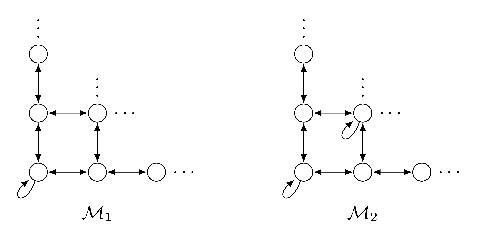
\includegraphics[scale=0.8]{figure1.eps}
\medskip
\caption{Two $\tle$-bisimilar models}\label{fig}
\end{center}
\end{figure}

We prove that $\model_1,0\bisim\model_2,0$
showing the winning strategy for duplicator. Intuitively, the strategy for Duplicator consists in the following idea: whenever one player is in $(\model_1,0)$ the other will be in $(\model_2,0)$ or $(\model_2,1)$, and
conversely whenever a player is in $(\model_1,n)$, $n>0$ the other will be in
$(\model_2,m)$, $m>1$. This is maintained until Spoiler (if ever) decides to
remember a state. Once this is done, then any strategy will be a winning one for Duplicator.


Being a bit more formal, the winning strategy will have two stages. While Spoiler does not remember any reflexive
state, Duplicator plays with the following strategy: if Spoiler
chooses $0$ in any model, Duplicator chooses $0$ in the other one;
if Spoiler chooses $n>0$ in $\model_1$, Duplicator plays $n+1$ in
$\model_2$; if Spoiler chooses $n>0$ in $\model_2$, Duplicator plays
$n-1$ in $\model_1$.

Notice that with this strategy Spoiler chooses
a reflexive state if and only if Duplicator answers with a reflexive
one. This is clearly a winning strategy. If ever Spoiler decides to
remember a reflexive state, Duplicator starts using the following
strategy: if Spoiler selects a state $n$, Duplicator answers with an
agreeing state $m$ of the opposite model. Notice that this is always
possible since both $n$ and $m$ see infinitely many non remembered
states and at least one remembered state. Therefore $\model_1,w \bisim \model_2, w$.

On the other hand, let $\varphi$ be the formula $\down i. \diam{r}(i \land \diam{r}(\lnot i \land \down i.\diam{r}i))$. It is easy to see that $\model_1, w \not \models \varphi$ but $\model_2, w \models \varphi$.
\end{pf}

The basic idea behind the previous proof is that if the relations
$R_1$ and $R_2$ extend the set $\{(n,m) \mid n\not= m\}$, then
$\tle$ can distinguish between irreflexive and non irreflexive frames,
but it cannot distinguish frames with a different number of reflexive nodes.

There is a number of interesting remarks to be made above the
previous proof. First, notice that it is essential for the winning
strategy of Duplicator that each state in a model is related to
infinitely many others.


We have already shown that $\tle \not= \hlogic$ and we used a pair
of infinite models to distinguish both logics. We now analyze the
question whether $\tle \not= \hlogic$ on image-finite models. We
prove that $\hlogic \not \leq \tle$ on image-finite models showing
that there cannot exist an equivalence preserving translation for
finite models from $\hlogic$ to $\tle$

\tb{below should not be a definition (it is only used in the proof of Theorem 10).
Give first the theorem and move the lemmas to 'claims' within the proof.  The
definition of the models goes also inside the proof.}

\begin{defn}
Let $\model^1_n = \diam{W_n, R_1, \emptyset, \emptyset}$ and
$\model^2_n = \diam{W_n, R_2, \emptyset, \emptyset}$, where
$W_n=\{w_0, \dots, w_{n-1}\}$, $R_1 = \{(n,m)\mid n \neq m\} \cup
\{(w_0,w_0)\}$ and $R_2 = \{(n,m)\mid n \neq m\} \cup \{(w_0,w_0)\}
\cup \{w_1, w_1\}$, with $n\geq 1$.
\end{defn}

\begin{lem}\label{lem:not-distinguish}
Let $\varphi$ be a $\tle$-formula such that the number of
occurrences of the $\remember$ operator is at most $n$. Then
$\model^1_{n+2}, w_0 \models \varphi$ iff $\model^2_{n+2}, w_0
\models \varphi$.
\end{lem}
\begin{pf}
We prove that Duplicator has a winning strategy in the game
$E(\model^1_{n+2},\model^2_{n+2}, w_0, w_0)$ in the case Spoiler
makes at most $n$ memorizing steps. The strategy for Duplicator is
the following. While Spoiler does not remember any reflexive state,
Duplicator plays with the following strategy: if Spoiler chooses
$w_0$ in any model, Duplicator chooses $w_0$ in the other one; if
Spoiler chooses $w_k$, $0 < k < n+1$, in $\model_1$, Duplicator
plays $w_{k+1}$ in $\model_2$, and if Spoiler chooses $w_{n+1}$ in
$\model_1$, Duplicator plays $w_2$ in $\model_2$; if Spoiler chooses
$w_k$, $k > 0$, in $\model_2$, Duplicator plays $w_{k-1}$ in
$\model_1$. Note that with this strategy, Spoiler chooses a
reflexive state iff Duplicator answers with a reflexive one. If ever
Spoiler decides to remember a reflexive state, then from that point
of the game, for every state $w_n$ chosen by Spoiler, Duplicator
will always have an agreeing state $w_m$ on the opposite model he
can choose. This happens because the models have $n+2$ states, and
therefore there is always at least two non-remembered states. That
means that both $w_n$ and $w_m$ see at least one remembered state
and at least one non-remembered state, and this condition will hold
for the rest of the game.
\end{pf}

\begin{lem}\label{lem:distinguish}
Let $\varphi = \down i. \diam{R}(i \land \diam{R}(\lnot i \land
\down i. \diam{R}i))$. For every $n \geq 1$, $\model^1_n, w_0
\not\models \varphi$ and $\model^2_n, w_0 \models \varphi$.
\end{lem}
\begin{pf}
Trivial.
\end{pf}

\begin{thm}
There is no translation $Tr$ from $\hlogic$-sentences to
$\tle$-formulas such that for every finite model $\model$ and every
formula $\varphi$ of $\hlogic$ we have $\model \models_{\hlogic}
\varphi$ iff $\model \models_{\tle} Tr(\varphi)$.
\end{thm}
\begin{pf}
Let us suppose that such translation $Tr$ exists. Let $\varphi$ a
$\hlogic$-formula as in Lemma~\ref{lem:distinguish}, and let $n$ be
the complexity of $Tr(\varphi)$. Because $Tr(\varphi)$ has at most
$n$ remember operators, we know by Lemma~\ref{lem:not-distinguish}
that $\model^1_{n+2}, w_0 \models Tr(\varphi)$ iff $\model^2_{n+2},
w_0 \models Tr(\varphi)$. But on the other hand, $\model^1_{n+2},
w_0 \not \models \varphi$ and $\model^2_{n+2}, w_0 \models \varphi$.
This is an absurd, since $Tr$ should be an equivalence preserving
translation for finite models.
\end{pf}




Second, notice that the $\hlogic$ sentence that we used in the proof
uses only one nominal.  Hence, we have actually proved that
$\hlogicone\not\le\tle$, where $\hlogicone$ is $\hlogic$ restricted
to only one nominal.  But actually, it is also the case that $\tle
\not\le\hlogicone$.

\tb{Give the general claim for an arbitrary $k$ as a theorem. Then
say that we just prove the case for $k=1$ and that the rest are similar.}
\begin{pro}\label{prop:hlogicone_incomparable_tle}
The logics $\hlogicone$ and {\em $\tle$} are incomparable in terms of expressive power.
\end{pro}

\begin{pf}
As we said, $\hlogicone\not\leq\tle$ is a direct consequence of the
proof of Theorem~\ref{thm:tle_not_equal_hlogic}. To prove $\tle \not
\le \hlogicone$, let $\model_1=\diam{\{1,2,3\},\{(i,j) \mid 1 \leq
i,j \leq 3\},\emptyset,\emptyset}$ (a clique of size 3) and
$\model_2=\diam{\{1,2\},\{(i,j) \mid 1 \leq i,j \leq
2\},\emptyset,\emptyset}$ (a clique of size 2). It is easy to check
that $\model_1,1 \bisim_{\hlogicone} \model_2,1$. However, the
formula $\varphi = \remember \diam{r} (\lnot\known \land \remember
\diam{r} (\lnot\known \land \remember \diam{r} \lnot\known))$
distinguishes the models: $\model_1,1 \models \varphi$ but
$\model_2,1 \not\models \varphi$.
\end{pf}

Actually, this incomparability result can be extended to $\hlogic$ restricted to any fixed number of nominals, by taking cliques of the appropriate size.

\begin{thm}
For any fixed $k$, the logics $\hlogick$ and {\em $\tle$} are incomparable in terms of expressive power.
\end{thm}
\medskip

\noindent
We will now briefly discuss the case of $\tl$.  As we already mentioned at the beginning
of this section, the first required step to compare expressivity is to be able to define
a natural mapping between models of the different logics involved.  Consider a model
$\diam{W,\rels,V,S}$ for $\tl$; if we want to associate a Kripke model we have to decide
how to deal with the set $S$.  The only natural choice seems to be to extend the signature
with a special propositional variable \emph{known}, and let $V'$ be identical to
$V$ excepts that $V'(\mathit{known}) = S$.  And  the same can be done to obtain a hybrid model
from a $\tl$ model.


\begin{thm}\label{thm:expr_power}
The following results concerning expressive power can be established
\begin{enumerate}
\item $\bml$ over the signature $\diam{\prop \cup \{\mathit{known}\}, \rel}$ is strictly
less expressive than {\em $\tl$} over the signature $\diam{\prop, \rel}$.
\item {\em $\tl$} over the signature $\diam{\prop, \rel}$ is strictly less expressive
than $\hlogic$ over the signature $\diam{\prop \cup \{\mathit{known}\}, \rel,\nom}$.
\item {\em $\tle$} over the signature $\diam{\prop \cup \{\mathit{known}\}, \rel}$ is equivalent to \linebreak
{\em $\tl$} over the signature $\diam{\prop, \rel}$
\end{enumerate}
\end{thm}

\begin{pf}
All proofs are similar to (and sometimes easier than) the ones
presented above. We only discuss 2. To prove $\tl \le \hlogic$ (over
the appropriate signatures) we adapt the translation $\Tr$ with the
following clause for $\known$
$$
\begin{array}{rcl}
\Tr_N(\known) & = & \big (\bigvee_{i \in N} i \big) \vee
\mathit{known}.
\end{array}
$$
$\hlogic \not \le \tl$ can be shown using the following models. Let
$\model_1=\diam{\{w\},$ $\{(w,w)\},\emptyset,\{w\}}$ and
$\model_2=\diam{\{u,v\},\{(u,v),(v,u)\},\emptyset,\{u,v\}}$.
Duplicator always wins on $E(\model_1,\model_2,w,u)$ and thus
$\model_1,w\bisim_{\tl}\model_2,u$. On the other hand,
$\model'_1,w\models_{\hlogic}\down i.\diam{r}i$ but
$\model'_2,u\not\models_{\hlogic}\down i.\diam{r}i$, for $\model'_1,
\model'_2$ the  models corresponding to $\model_1$ and $\model_2$.
\end{pf}

To close this section, we mention that the satisfaction preserving translations defined in
the proof can actually be used to transfer known results, for example, from  $\hlogic$ to $\tl$ and $\tle$.  For
instance, both logics are compact and their formulas are preserved by generated submodels (see~\cite{areces01:_hybrid}).
